\documentclass[11pt]{article}
\usepackage[letterpaper, left=.8in, top=0.9in, right=.8in, bottom=0.70in,nohead,includefoot, verbose, ignoremp]{geometry}
%\usepackage{charter} %choose default font ... your choice here % {mathptmx} % mathrsfs} % mathptmx} %mathpple} %mathpazo}
\usepackage[round]{natbib}
\usepackage{enumerate} % for different labels in numbered lists 
%\usepackage{xy}\xyoption{all} \xyoption{poly} \xyoption{knot}  
\usepackage{latexsym,amssymb,amsmath,amsfonts,graphicx,color,amsthm,enumerate,natbib,mathtools, bm, float} %,fancyvrb,movie15
\usepackage{dsfont}
\usepackage[pdftex,pagebackref=true]{hyperref}
\usepackage[svgnames,dvipsnames,x11names]{xcolor}
\hypersetup{
colorlinks,%
linkcolor=RoyalBlue2,  % colour of links to eqns, tables, sections, etc
urlcolor=Sienna4,   % colour of unboxed URLs
citecolor=RoyalBlue2  % colour of citations linked in text
}
\pagestyle{empty} % no page number on front page
\usepackage{todonotes}
%\usepackage{mathrsfs} % For \mathscr function

%\renewcommand{\includegraphics}{}  % use this to suppress inclusion of figs for proofing

% custom definitions ...
\def\eq#1{equation (\ref{#1})}
\def\pdf{p.d.f.\ } \def\cdf{c.d.f.\ }
\def\pdfs{p.d.f.s} \def\cdfs{c.d.f.s}
\def\mgf{m.g.f.\ } \def\mgfs{m.g.f.s\ }
\def\ci{\perp\!\!\!\perp}                        % conditional independence symbol
\def\beginmat{ \left( \begin{array} }
\def\endmat{ \end{array} \right) }
\def\diag{{\rm diag}}
\def\log{{\rm log}}
\def\tr{{\rm tr}}
\def\etr{{\rm etr}}
\def\Ei{{\rm Ei}}
\def\cD{\mathcal{D}}
\def\cS{\mathcal{S}}
\def\cM{\mathcal{M}}
%\newtheorem{thm}{Theorem}
\newcommand{\Reals}{\mathbb R}
\newcommand{\Beta}{\mathrm{Beta}}
\newcommand{\KL}{\mathrm{D}_{KL}}
\newtheorem{thm}{Theorem}[section]
\newtheorem{lemma}{Lemma}[section]
\newcommand{\df}{\vcentcolon=}
\newcommand{\ex}{{\mathbb E}}
\newcommand{\pfrac}[2]{\left(\frac{#1}{#2}\right)}

\DeclareBoldMathCommand{\balpha}{\alpha}
\DeclareBoldMathCommand{\bbeta}{\beta}
%

%%My Definitions
\def\qed{\hfill $\square$}
\newcommand{\indep}{\mathop{\perp\!\!\!\!\perp}}

\def\ts{\tilde{s}}

%% Document starts here ...
%%
\begin{document}
\vspace{-1in}
\title{A Sequential Hypothesis Test for Implementation Errors and Missing Data in Simply Randomized Experiments}
\author{\Large Michael Lindon \\ Optimizely \and Alan Malek \\ Optimizely?}
\maketitle 
%\centerline{{\color{RoyalBlue2}{Due: someday.}}}\bigskip
%\thispagestyle{empty}
\begin{abstract}
  Simply randomized designs are one of the most common controlled experiments used to study causal effects.
  Failure of the assignment mechanism, to provide proper randomization of units across treatments, or the data collection mechanism, when data is ``missing not at random'', can render subsequent analysis invalid if not properly identified. In this paper we demonstrate that such practical implementation errors can often be identified, fortunately, through consideration of the total unit counts resulting in each treatment group.
  Based on this observation, we introduce a sequential hypothesis test constructed from Bayesian Multinomial-dirichlet families for detecting practical implementation errors in simply randomized experiments. By establishing a Martingale property of the posterior odds under the null hypothesis, frequentist Type-I error is controlled under both optional stopping and continuation via maximal inequalities, preventing practitioners from potentially inflating false positive probabilities through continuous monitoring.
  In contrast to other statistical tests which are performed once all data collection is completed, the proposed test is sequential - frequently rejecting the null during the process of data collection itself, saving further units from entering an improperly-executed experiment.
  We illustrate the utility of this test in the context of online controlled experiments (OCEs), where assignment is automated through code and data collected through complex processing pipelines, often in the presence of unintended bugs and logical errors. Confidence sequences posessing nominal sequential frequentist coverage probabilities are provided and their connection to the Bayesian support interval is examined. The differences between the pure Bayesian and sequential frequentist testing procedures are finally discussed through a conditional frequentist testing perspective.  
\end{abstract}


\section{Introduction}
\label{sec:intro}
Randomized treatment assignment satisfies many purposes in controlled experiments (see \cite{kempthorne}, \cite{cox} and \cite{rubin}). Arguably the least controversial justfication is the attempt to remove any personal, systematic or selection bias in the treatment assignment mechanism, although this is neither without criticism nor without alternative (see \cite{lindley} and \cite{kadane}). Consider for example a medical researcher who selects patients most likely to recover to receive her preferred experimental drug. Without explicitly conditioning on this information in the assignment mechanism, causal estimands such as the average treatment effect may be biased, overestimating the efficacy of the new drug (\cite{berry}).
Simply randomized experiments attempt to remove the possibility of bias by randomly assigning experimental units independently to treatment groups with a constant probability vector.
This design is useful in contexts where units enter the experiment sequentially, as opposed to being simultaneously available like in completely randomized designs, and are often used in the technology industry to run online controlled experiments (OCEs) (\cite{oce}). Formally let there be $d$ treamtent groups, $\theta_0 \in \mathcal{S}^d$ be a probability vector where element $\theta_{0,i}$ denotes the probability of any unit being assigned to treatment group $i$, and $x_j$ a random variable denoting the assignment outcome of the $j'th$ experimental unit. The simply randomized design can then be summarized by the following probabilistic assignment mechanism
\begin{equation}
  \label{eq:multinomialassignment}
  x_1,x_2, \dots \sim \text{Multinomial}(1,\theta_0).
\end{equation}
The statistician may not be personally involved with the data collection process and may simply be told the assignment mechanism after being presented with the data for analysis. The observant statistican has a right for concern, therefore, when they are provided with data which does not support the purported assignment mechanism. For simply randomized experiments the total unit counts assigned to each treatment group can provide evidence against equation \eqref{eq:multinomialassignment}.
Indeed this is a strong indicator that the experiment has not been conducted as expected, either through a biased assignment mechanism depending on unreported covariates which the statistician cannot control for, or through an unintential missing data mechanism in the collection and reporting process, which could depend on the outcome being meaured such as censoring or other ``missing not at random'' (MNAR) mechanisms (\cite{missing-data}).
Such observations occurs frequently in OCEs and are colloquially referred to in the technology industry as \textit{sample ratio mismatches} (SRMs).

OCEs automate the assignment mechanism through code and instrument data collection and cleaning through complex transformtions which often introduce bugs and logical errors. It is unsurprising, therefore, that \cite{fabijan} reports that 6\% of all experiments performed in a at Microsoft contained bugs which were revealed by SRMs. The authors describe in detail the engineering architecture required for assignment and data collection in OCEs and highlight how SRMs frequently reveal bugs therein. An example a simple experiment to study user engagement on an improved version of a web page is provided. Not all visitors to a web page are human, however, and data must be cleaned to remove non-human interactions with the page, such as from web crawlers and scrapers. Unfortunately the classification between human and non-human visitors is performed algorithmically, and some users in the treatment group were so engaged with the new page that they were accidentally classified as non-human and removed prior to the analysis - essentially removing units most in favour of the treatment, resulting in fewer units than expected being reported in the treatment group. This is not an issue with the assignment mechanism, but in the data collection. It is an example of a \textit{censoring} missing data mechanism, a special case of MNAR.

\cite{zhao} describes an example in which the user identifer becomes lost, preventing users from receiving a consistent experience over time, with some users initially assigned to the treatment becoming exposed to and recorded in the control - an example of noncompliance (\cite{imbens}). 

Many other practical abnormalities can be revealed by considering the total counts in each treatment group after collection. For this reason an industry best practise has evolved where practitioners run a Chi-squared test against the null in equation \eqref{eq:multinomialassignment}, after data collection has finished and prior to analysis, to test the validity of the collected data \cite{linkedin}.
The authors note two deficiencies of this check. The first deficiency, and most obvious, is that one learns about a problem in the data only after data collection has completed. It ia ssumed that there is an implicit cost of including a unit in an experiment, and so ideally one would like to learn about such problems as soon as possible to prevent further units from entering an improperly executed-experiment. The second deficiency, and motivated from the first, is that this encourages practitioners to incorrectly \textit{continuously monitor} their experiments through the repeated application of significance tests without any multiplicity correction (\cite{armitage}).

In order to develop a test that performs well under optional stopping and continuation the authors take inspiration from Bayesian methods satisfying the \textit{stopping rule principle}, that the reason for stopping an experiment should be irrelevant to the hypothesis being tested, which follows from the likelihood principle \cite{likelihood}. The contributions of this paper focus, however, on obtaining frequentist properties of such a sequential test.
The paper is outlined as follows. Section \ref{sec:srm_testing} defines a common Bayesian test through conjugate multinomial-Dirichlet models. Section \ref{sec:theory} establish the Martingale properties of the posterior odds under the null hypothesis, enabling a modified test to be developed which controls frequentist Type-I error probabilities below a nominal value under both optional stopping and continuation through maximal inequalities.  This safely permits the online testing of hypothesis \eqref{eq:multinomialassignment} after every single observation, without inflating frequentist false positive probabilities, with the obvious advantage of being able to safely reject the null and discover a practical implementation error early in the beginning of an experiment - preventing experimental units being wasted on a faulty experiment. Instance-specific upper-bounds on time-to-rejection are provided in terms of the KL divergence  between $\theta_0$ and the actual generating distribution of the samples. This sequential test is then inverted to define confidence sequences which possess nominal frequentist coverage probabilities. Section \ref{sec:simulation} presents a number of simulation studies illustrating how false positive probabilities are dramatically inflated through the repeated significance testing using a Chi-squared test compared to the guarantees afforded by the proposed test, in addition to how quickly the proposed test is able to reject the null when it is invalid. The final section \ref{sec:discussion} connects these contributions with existing literature. In particuar, the confidence sequence defined in \ref{sec:theory} is identified as the Bayesian support interval of \cite{support_interval} through an application of the Savage-Dickey density ratio. The differences between the pure Bayesian test and the proposed test are discussed from the perspective of conditional frequentist testing (\cite{conditional_frequentist_simple}, \cite{conditional_frequentist_precise}, \cite{conditional_frequentist_composite}).




%When a sample ratio mismatch is observed in an experiment and the difference is believed to be caused due to missing data, practitioners are neither willing to assume the missingness process is ignorable, nor are willing to model the missingness. The reluctance to model the missingness process is understandable because there are simply too many mechanisms by which data could be lost, which will be the focus of section \ref{causes_of_srms}, too many experiments being performed and OCEs are relatively cheap. It is far more common to test for an SRM and simply repeat the experiment after correcting the bug. Testing for SRMs is the focus of section \ref{srm_testing} 

\section{Sequential Bayesian Multinomial Test}
\label{sec:srm_testing}
The assignment outcome of an experimental unit to a treatment group is a $\text{Categorical}(\theta)$ random variable with the allocation probabilities $\theta=\theta_0$ the specified as part of the design. Practitioners may not, however, have such granularity. They may know, instead, only the number of units allocation to each treatment group after certain intervals, such as every hour or day etc. For this reason it is helpful to express the problem as observing a sequence of multinomial random variables $x_i \sim \text{Multinomial}(n_i, \theta)$, which naturally provides observations after every unit assignment a special case with $n_i = 1$. The likelihood doesn't change however, and so neither does the analysis.
The sequentially recorded observations may differ from this null hypothesis, which we will denote $M_0$, if there is an unintended bias in the assignment mechanism or if an unknown missing data mechanism, as discussed in section \ref{sec:intro}.

To develop a Bayesian hypothesis test it is necessary to specify an alternative model for the data, denoted $M_1$. Consider the following model studied in \cite{good},
\begin{align}
    x_i | \theta, M_1 &\sim \text{Multinomial}(n_i,\theta), \hspace{1cm} \text{independently for }\, i=1,2,\dots\\
  \theta | M_1 &\sim \text{Dirichlet}(\alpha_0).\notag
\end{align}
Prior mass is concentrated aroound $\theta_0$ by specifying $\alpha_{0,i} = k \theta_{0,i}$ for concentration parameter $k \in \mathbb{R}^+$, in line with a ``Jeffreys-type'' testing procedure - for if the null weren't at least somewhat plausible, then a statistical test wouldn't be needed. The Bayes factor comparing models $M_1$ to $M_0$ is analytically tractable and is given by

\begin{equation}
  \label{eq:bayes_factor}
 BF_{10}(x_{1:t}) = \frac{p(x_{1:t}|M_1)}{p(x_{1:t}|M_0)} = \frac{\Gamma(\sum_{j=1}^{d} \alpha_{0,j})}{\Gamma(\sum_{j=1}^{d} \alpha_{0,j} + \sum_{i=1}^{t}x_{i,j})}\frac{\prod_{j=1}^{d}\Gamma(\alpha_{0,j} + \sum_{i=1}^{t}x_{i,j} )}{\prod_{j=1}^{d}\Gamma(\alpha_{0,j} )}\frac{1}{\prod_{j=1}^{d} \theta_{0,j}^{\sum_{i=1}^{t}x_{i,j}}},
\end{equation}
which, when combined with the prior odds, yields the posterior odds of model $M_1$ to $M_0$.
It is helpful, however, to consider the posterior odds as computed sequentially through the following recursive definition,
\begin{equation}
  \label{eq:update_rule}
  O_{t}(\theta_0) = \frac{\Gamma(\sum_i \alpha_{t-1,i})}{\Gamma(\sum_i \alpha_{t-1,i} +  x_{t,i})} \frac{\prod_i \Gamma(\alpha_{t-1,i} + x_{t,i})}{\prod_i \Gamma(\alpha_{t-1,i})} \frac{1}{\prod_i \theta_{0,i}^{x_{t,i}}}  O_{t-1}(\theta_0).
\end{equation}
where $\alpha_t = \alpha_{t-1}+x_t$ and $O_0(\theta_0)=p(M_1)/p(M_0)$ (see appendix section \ref{app:posterior_odds}). In the rest of this paper we will always assume that the prior odds are unity, and so posterior odds are interchangeable with Bayes factors. Recursive definitions, however, require an initial value and for that reason we choose to work with the posterior odds. The dependence of $O_t(\theta_0)$ on the observed data $x_{1:t}$ is implicit in this notation, yet the null value $\theta_0$ being tested is made explicit to aid the discussion of confidence sequences in theorem \ref{thm:confidence_sequence}. If $\alpha_0$ is integer valued, and observations occur after every unit assignment ($n_i=1$) so that all but one of the $x_{t,j}$ is 1 with the others 0, the recursive definition simplifies substantially to
\begin{align}
  \label{eq:simplified_bayes_factor}
  O_{t}(\theta_0) &= \prod_{j=1}^{d} \left(\frac{\alpha_{t-1,j}}{\sum_i \alpha_{t-1,i}} \frac{1}{\theta_{0,j}}\right)^{x_{t,j}} O_{t-1}(\theta_0),\\
  &=\prod_{j=1}^{d}\left(\frac{E[\theta_j|x_{1:t-1}]}{\theta_{0,j}} \right)^{x_{t,j}} O_{t-1}(\theta_0),
\end{align}
where the last line follows from the mean of the Dirichlet posterior predictive distribution. This multiplicative update has some intuitive appeal - it is the expected probability, based on our current Bayesian belief, divided by the null probability of the event that occured.
A pure Bayesian analysis could proceed by rasing an alert when $O_t(\theta_0) > c$ and reporting a subjective error probability of less than $1/(1+c)$ (see chapter 5 of \cite{bernardo}).
Many would argue, however, that it is not possible to develop a subjective prior on the $\theta$ resulting from a practical implementation error if one were to exist (although it is our experience across multiple experiments that the resulting $\theta$ is usually very close to $\theta_0$).
We instead, therefore, develop a test based on $O_t(\theta_0)$ which controls the frequentist Type-I error under optional stopping and continuation, regardless of the choice of $\alpha_0$.
\section{Theoretical Results}
\begin{thm}(Uniform Bound on Posterior Odds under Null)
  
  \label{thm:type_1_error}
\noindent Let $x_i,$ be a sequence of $\text{Multinomial}(n_i,\theta)$ random variables and consider the sequence of posterior odds $O_t(\theta_0)$ defined as in equation \eqref{eq:update_rule} with $O_0(\theta_0)=1$, then
\begin{equation}
  \label{eq:type_1_error}
  \mathbb{P}_{\theta = \theta_0}\left( \exists t \in \mathbb{N}: O_t(\theta_0) \geq 1/u \right) \leq u,
\end{equation}
for all $u \in [0,1]$ and for all choices of $\alpha_0$. 
\end{thm}
\noindent The uniform condition in equation \ref{eq:type_1_error} suggests the stopping rule $\tau = \inf \lbrace t \in \mathbb{N}: O_t(\theta_0) \geq 1/u \rbrace$ for rejecting the null hypothesis. Simply stated, a practitioner who rejects the null hypothesis as soon as the posterior odds become larger than $1/u$ incurs a frequentist type-I error probability of at most $u$. The proof, based on Martingale maximal inequalities, can be found in appendix section \ref{app:type_1_error}. Results of this form can be found in the literature as early as \cite{ville}. An alternative and succinct proof, with applications to the special case of Binomial-Uniform families, can be found in section 1 of \cite{robbins}. Furthermore, the posterior odds are equal to the Bayes factor under prior odds of unity, and so theorem \ref{thm:type_1_error} can also be established as a corrolary of mixture sequential probability ratio test of \cite{wald}. In the words of Wald, the alternative likelihood divided by the null likelihood is integrated w.r.t. a \textit{weight} function over the unknown parameter, and the hypothesis is rejected as soon as the mSPRT test statistic exceeds $1/u$ in order to obtain a Type-I error of at most $u$. It is plain to see that when the weight function is the prior distribution, then the mSPRT test statistic is simply the Bayes factor, and that results of this kind can be established for other Bayesian  simple null vs composite alternative hypothesis tests. In the language of \cite{johari} one can define a conservative sequential p-value process by
\begin{align}
  p_t &= \min(p_{t-1}, 1/O_t(\theta_0)),\\
  p_0 &=1,
\end{align}
which satisfies the following sequential analogue of a conservative p-value
\begin{equation}
  \label{eq:conservative_p_value}
  \mathbb{P}_{\theta = \theta_0}\left( \exists t \in \mathbb{N}: p_t \leq u \right) \leq u.
\end{equation}
Further connections between sequential p-value processes and Bayes factors are discussed in \cite{shafer}.
The following theorem exploits the duality between p-values and confidence intervals to derive sequential confidence sequences.
\begin{thm}(Confidence Sequences)
  
  \label{thm:confidence_sequence}
  \noindent Under the assumptions of theorem \ref{thm:type_1_error} let $I_t(u) = \lbrace \theta \in \mathbb{S}^d : O_t(\theta) < 1/u  \rbrace$, then
\begin{equation}
  \label{eq:confidence_sequence}
  \mathbb{P}_{\theta}\left( \theta \in \bigcap_{t=1}^{\infty} I_t(u) \right) \geq 1- u,
\end{equation}
for all $u \in [0,1]$ and for all choices of $\alpha_0$. 
\end{thm}
\noindent Each $I_t(u)$ is a convex subset of $\mathbb{S}^d$. If confidence sequences on individual components of $\theta$ are desired, however, then one can solve the following
optimization problems
\begin{align*}
  &\text{Maximize/Minimize} &\theta_i, &\\
  &\text{subject to}  &ku &< \prod_{j=1}^{d} \theta_{0,j}^{\sum_{i=1}^{t}x_{i,j}},\\
    &              &\sum_{i=1}^{d}\theta_i &= 1,\\
  &\text{where} &k &= \frac{\Gamma(\sum_{j=1}^{d} \alpha_j)}{\Gamma(\sum_{j=1}^{d} \alpha_j + \sum_{i=1}^{t}x_{i,j})}\frac{\prod_{j=1}^{d}\Gamma(\alpha_j + \sum_{i=1}^{t}x_{i,j} )}{\prod_{j=1}^{d}\Gamma(\alpha_j )}.
\end{align*}
The objective is linear, while the constraints defining the feasible set $I_t(u)$ are convex and linear respectively, resulting in a convex optimization problem. Let $j^{u}_{t,i}(u)$ and $j^{l}_{t,i}(u)$ be the solution to the maximization and minimization of $\theta_i$ over $I_t(u)$ and let $J_{t,i}(u)=[j^{l}_{t,i}(u), j^{u}_{t,i}(u)]$, then
\begin{equation}
  \label{eq:marginal_confidence_sequence}
  \mathbb{P}_{\theta}\left( \theta_i \in \bigcap_{t=1}^{\infty} J_{t,i}(u),\, \text{for}\, i = 1,2, \dots, d \right) \geq 1- u.
\end{equation}
These provide intervals which posess a nominal frequentist coverage probability for all time $t$ over all components simultaneously. 

Control over Type-I error probabilities would be of little value if the test were to have little ability to reject the null when $\theta \neq \theta_0$. To prove that this test is not trivial, we prove that the test rejects the null when $\theta \neq \theta_0$ almost surely, or that the test is asymptotically power 1 in the words of \cite{robbins}. We first establish the following result for the consistency of the posterior odds

\begin{thm}(Asymptotic Properties of Posterior Odds)
  
  \label{thm:consistency}
\noindent Let $x_i,$ be a sequence of $\text{Multinomial}(n_i,\theta_{\star})$ random variables with $\theta_{\star} \neq \theta_0$ and consider the sequence of posterior odds $O_t(\theta_0)$ defined as in equation \eqref{eq:update_rule} with $O_0(\theta_0)=1$, then
\begin{equation}
  \label{eq:consistency}
  \frac{1}{t} \log O_t(\theta_0) \rightarrow D_{KL}(\theta_{\star} || \theta_0) \hspace{1cm} a.s.
\end{equation}
as $t \rightarrow \infty$, for all choices of $\alpha_0$. 
\end{thm}
\noindent When $\theta_{\star} \neq \theta_0$, $D_{KL}(\theta_{\star} || \theta_0) > 0$, and so theorem \ref{thm:consistency} can be restated as $O_t(\theta_0) \rightarrow \infty$ almost surely as $t \rightarrow \infty$, which consequently rejects the null almost surely for any choice of Type-I error probability $u$. The formal proof is given in appendix section \ref{app:asymptotics}, which relies on theorem 1 of \cite{walker}, but the following hand-waving argument can provide much intuition. It is helpful to express the Bayes factor comparing $M_1$ to $M_0$ in terms of two seperate Bayes factors - the first comparing $M_{\star}$ to $M_1$ and the second comparing $M_{\star}$ to $M_0)$ as follows
\begin{align*}
 \frac{1}{t} \log BF_{10}(x_{1:t}) = - \frac{1}{t}\sum_{i=1}^{t}\log \left( \frac{p(x_{i}|M_\star)}{p(x_{i}|x_{1:i-1},M_1)}\right) + \frac{1}{t}\sum_{i=1}^{t} \log  \left( \frac{p(x_{i}|M_\star)}{p(x_{i}|M_0)}\right),\\
\end{align*}
where  $p(x_i|M_\star)$ is the density of a $\text{Multinomial}(n_i,\theta_{\star})$ distribution.
When the $x_i$ are independently distributed according to $\text{Multinomial}(n_i, \theta_\star)$, i.e. under model $M_\star$, then the second term converges to the Kullback-Leibler divergence between models $M_\star$ and $M_0$ by the strong law of large numbers. To adress the first term, note that as $t$ becomes large the dirichlet posterior $p(\theta|x_{1:t}, M_1)$ concentrates mass on $\theta_\star$, consequently bringing the posterior predictive $p(x_{t+1}|x_{1:t},M_1) =\int p(x_{t+1}|\theta,M_1),p(\theta|x_{1:t},M_1) d\theta$ closer to the ``true'' density $p(x_{t+1}|M_{\star})$. For $t$ large the logarithm of the fraction of densities becomes zero, and these zero terms then overwhelm the earler non-zero terms in the sum. We empirically illustrate this theorem in the next section.

\section{Simulation Studies}
\label{sec:simulation}
Consider null and true parameter value of $\theta_0=[1/2, 1/4, 1/4]$ and $\theta_\star=[1/2, 1/8, 3/8]$ respectively. The Kullback Leibler divergence of the null from the true multinomial distribution is $D_{KL}(p(\cdot|\theta_\star)||p(\cdot||\theta_0)) = 0.0654$ (to 4dp). A simulation of 1 million data points with $x_i \sim \text{Multinomial}(1, \theta_\star)$ and a Dirichlet prior with $\alpha_0 = 100\theta_0$ was used. The values of $\log(BF_{10}(x_{1:t}))/t$ were computed and are shown in figure \ref{fig:lbf}. The figure illustrates the convergence as described in theorem \ref{thm:consistency} of $\log(BF_{10}(x_{1:t}))/t$ to the Kullback Leibler divergence of the null from the true multinomial distribution.
\begin{figure}[H]
  \centering
  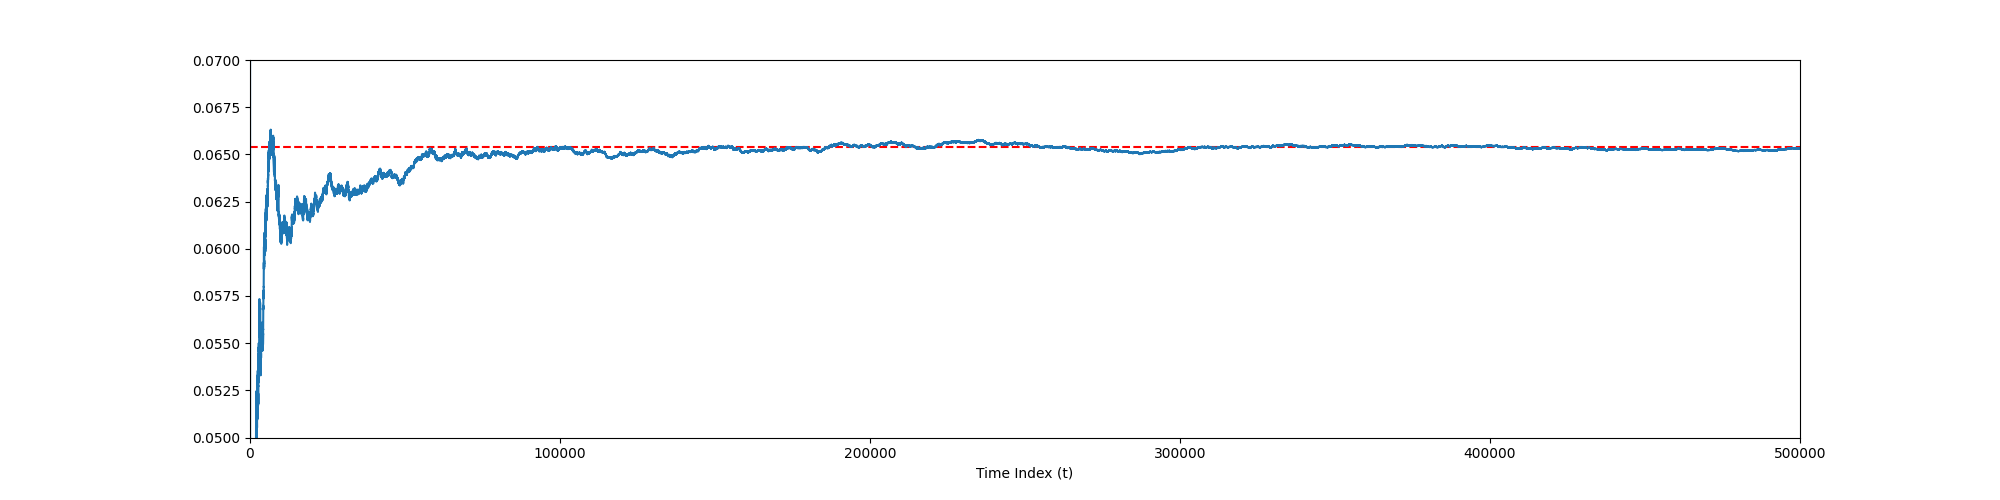
\includegraphics[scale=0.35]{images/consistency.png}
  \caption{Consistency of Bayes factor. The blue line shows $\log(BF_{10}(x_{1:t}))/t$ and the red dashed line shows $D_{KL}(p(\cdot|\theta_\star)||p(\cdot||\theta_0)) = 0.0654$.}
    \label{fig:lbf}
  \end{figure}
  In the following simulation we demonstrate the control over false positives provided by the proposed test. In addition, we demonstrate how continuously monitoring experiments can result in an incredibly large number of false positives when misusing a Chi-squared test. This is easiest to visualize in an example with one treatment group with assignment probability denoted $\rho$. The assignment is therefore a $\text{Bernoulli}(\rho)$ random variable, but sticking with the general framework developed earlier, the assignment outcome is $\text{Multinomial}(1,\theta)$ random variable with $\theta = [1-\rho, \rho]$. The Bayes factor in this case is then just a function of the sufficient statistic $\sum_{i=1}^t x_{i,1}$, or equivalently, $\hat{\rho}(x_{1:t}) = 1/t \sum_{i=1}^{t} x_{i,1}$, given by
\begin{equation}
  \label{eq:bayes_factor}
 BF_{10}(x_{1:t})  = \frac{\Gamma(\alpha_{0,0}+\alpha_{0,1})}{\Gamma(\alpha_{0,0}+\alpha_{0,1}+t)}\frac{\Gamma(\alpha_{0,0} + t-t\hat{\rho}(x_{1:t} ))\Gamma(\alpha_{0,1} + t\hat{\rho}(x_{1:t} )) }{\Gamma(\alpha_{0,0} )+\Gamma(\alpha_{0,1} )}\frac{1}{\theta_{0,0}^{t-t\hat{\rho}(x_{1:t})}\theta_{0,1}^{t\hat{\rho}(x_{1:t})}}.
\end{equation}
  Rejection of the null when the posterior odds $O_t(\theta_0)$ exceeds $1/u$, is equivalent to rejecting the null whenever the test statistic $\hat{\rho}(x_{1:t})$ falls outside a certain interval. This interval for $\theta_0 = [1/2,1/2]$, $\alpha_0 = 100*\theta_0 $, and $u=0.05$ is shown along with the interval for the Chi-squared test is shown in figure \ref{fig:critical}.
\begin{figure}[H]
  \centering
  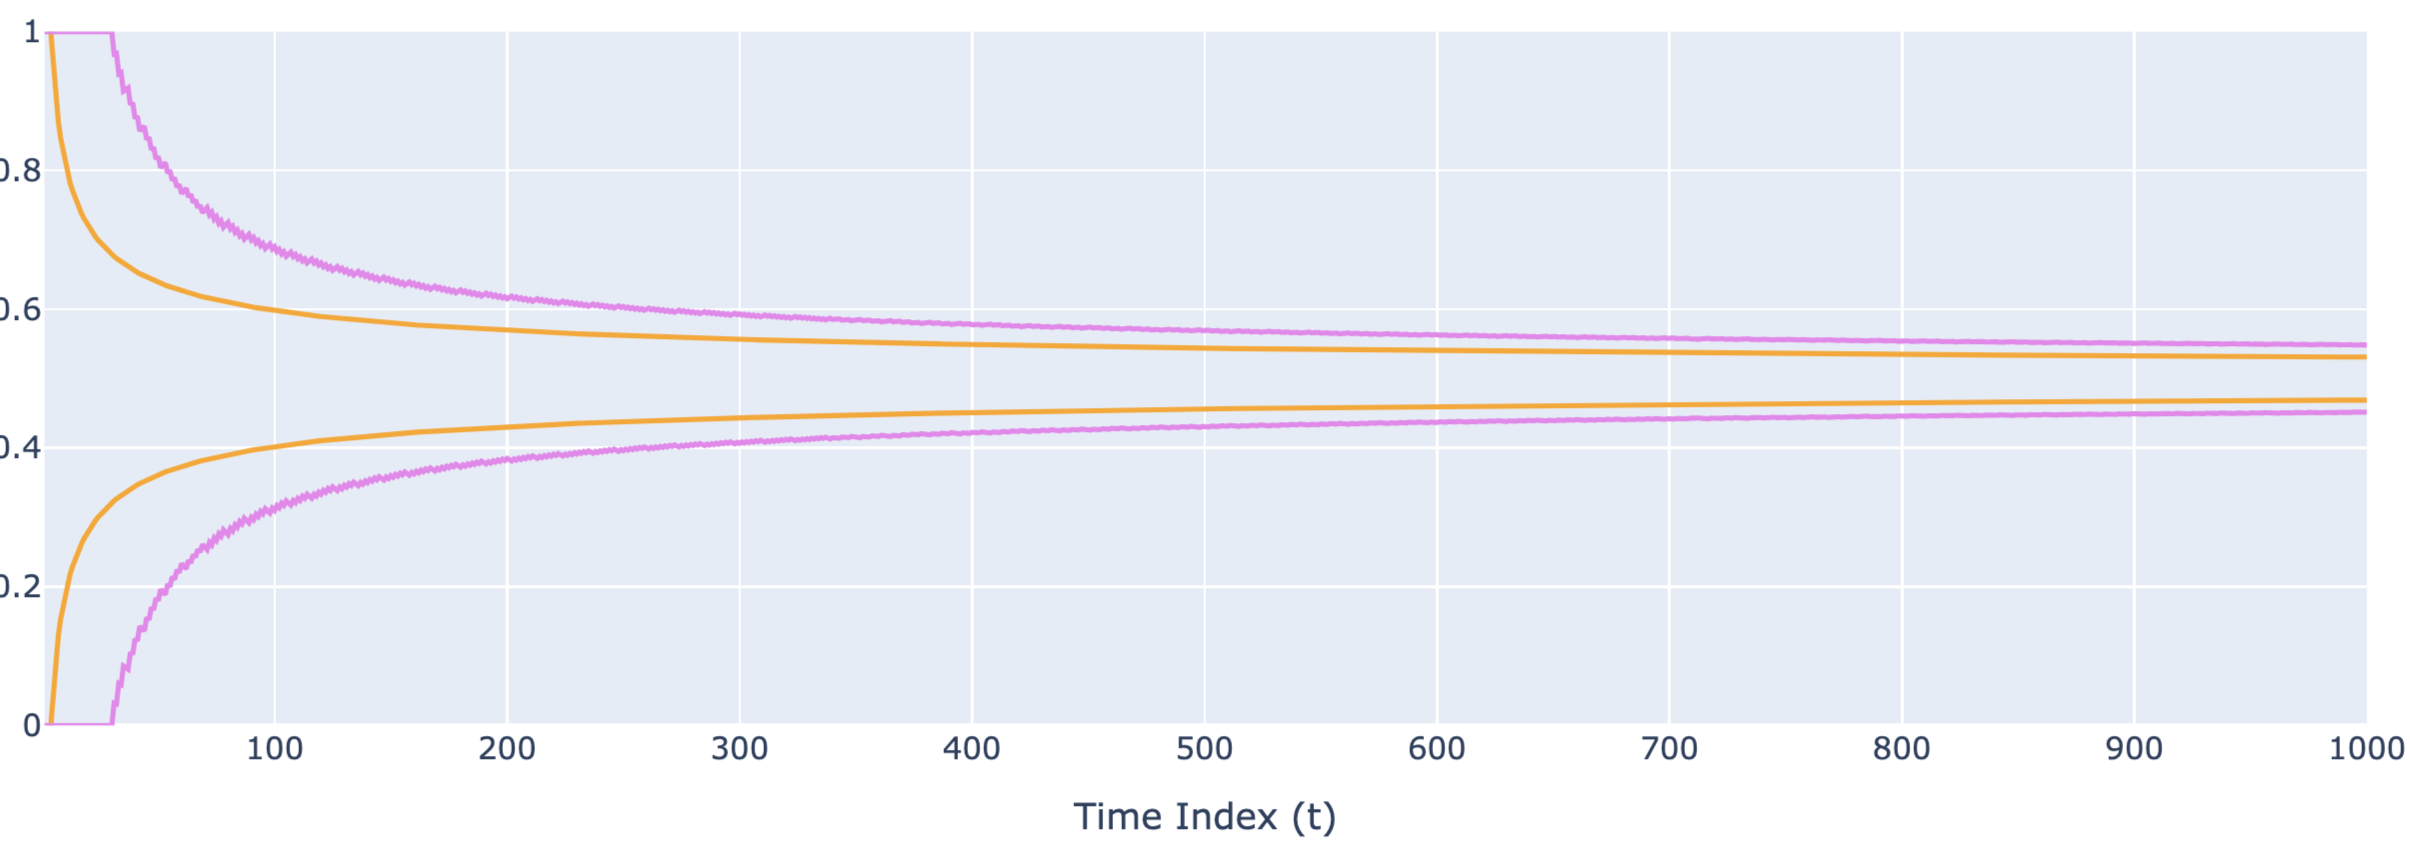
\includegraphics[scale=0.35]{images/critical_regions.png}
  \caption{Rejection boundaries for the proposed test ($\alpha_0 = 100\theta_0$) in magenta and the Chi-squared test in orange for testing the null hypothesis $\theta_0 = [0.5, 0.5]$ at a $u=0.05$ level. }
    \label{fig:critical}
  \end{figure}
  An important observation is that the rejection region at any time $t$ for the proposed test is a subset of that of the Chi-squared test. In other words, the Chi-squared test would declare a result ``significant'' at the $u=0.05$ level ``sooner'' than the proposed test. This has to be the case, for if the proposed test were significant as often as the Chi-squared test, then the proposed test would have just as many false positives under continuous monitoring.
  
  To illustrate this point further, 100 datasets were simulated under the null hypothesis up to $t=1000$. The Chi-squared ($u=0.05$) test was applied after every observation and by $t=1000$ 44 out of the 100 datasets resulted in the erroneous rejection of the null hypothesis. If left to run for longer, the total number of false positives would surely increase beyond 44. This is shown in figure \ref{fig:chi_fp}.
  \begin{figure}[h!]
  \centering
  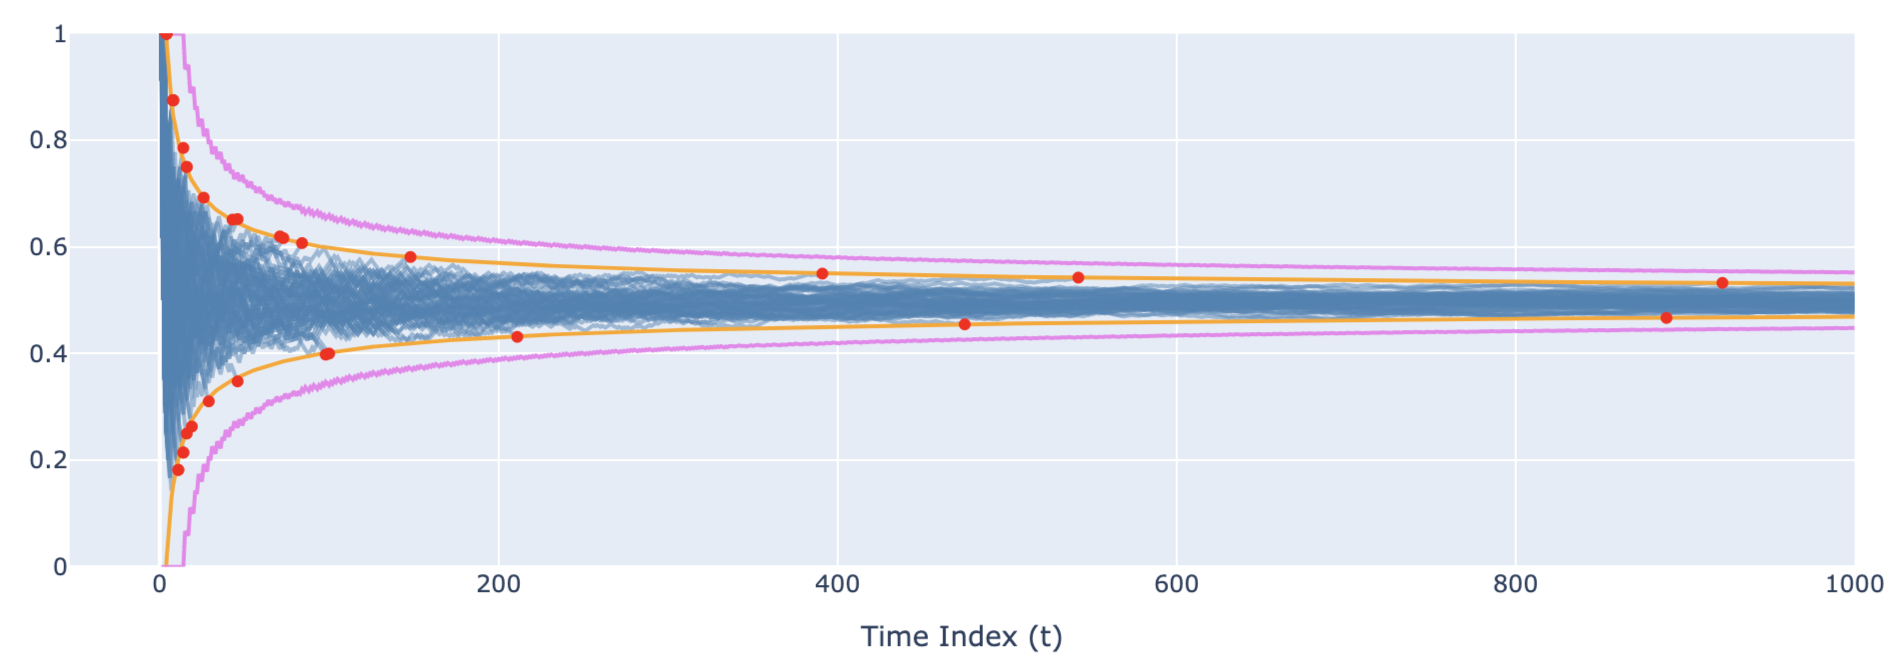
\includegraphics[scale=0.5]{images/chi_fp.png}
  \caption{Simulation Study of False Positives produced by continuously monitoring with a Chi-squared test. The orange and magenta curves are the same as in figure \ref{fig:critical}. Each blue trace is an independent simulation of $\hat{\rho}(x_{1:t})$ up until $t=1000$ or the first $t$ for which it crosses the rejection boundary of the Chi-squared test,visualized with a red dot, whichever comes sooner. }
    \label{fig:chi_fp}
  \end{figure}
  The simulation can be repeated, using the same random number seed, to demonstrate the control over false positives of the proposed test. Under identical conditions, the proposed test resulted in 2 out of 100 false positives, illustrated in figure \ref{fig:ssrm_fp}.
    \begin{figure}[H]
  \centering
  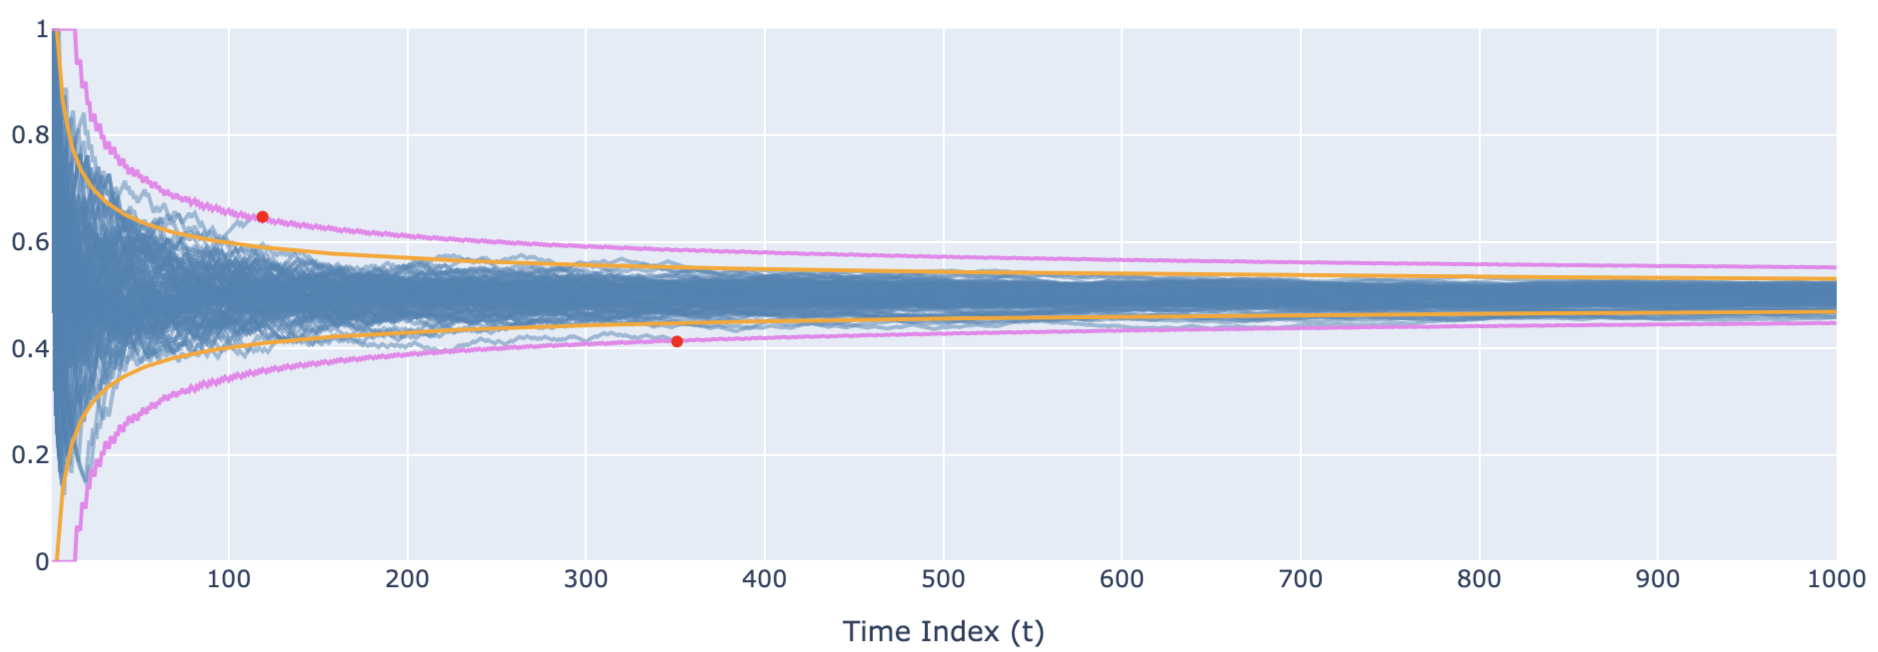
\includegraphics[scale=0.5]{images/ssrm_fp.png}
  \caption{Simulation Study of False Positives produced by continuously monitoring with the proposed test. The orange and magenta curves are the same as in figure \ref{fig:critical}. Each blue trace is an independent simulation of $\hat{\rho}(x_{1:t})$ up until $t=1000$ or the first $t$ for which it crosses the rejection boundary of the Chi-squared test,visualized with a red dot, whichever comes sooner. }
    \label{fig:ssrm_fp}
  \end{figure}
  We now turn our attention to visualizing the main value add of the proposed test, namely, to reject the null hypothesis quickly. Suppose an experiment has been designed and a sample size calculation has determined that $1000$ datapoints must be collected. The intended treatment assignment probability is 0.5, yet due to a bug in the code introducing bias in the assignment mechanism, or a missing data mechanism for the control group, the probability of recording an observation from the treatment is in fact 0.6.
  Figure \ref{fig:ssrm_reject} demonstrates that the proposed test rapidly rejects the null way before the end of the experiment, saving further units from entering an incorrectly executed experiment.
      \begin{figure}[H]
  \centering
  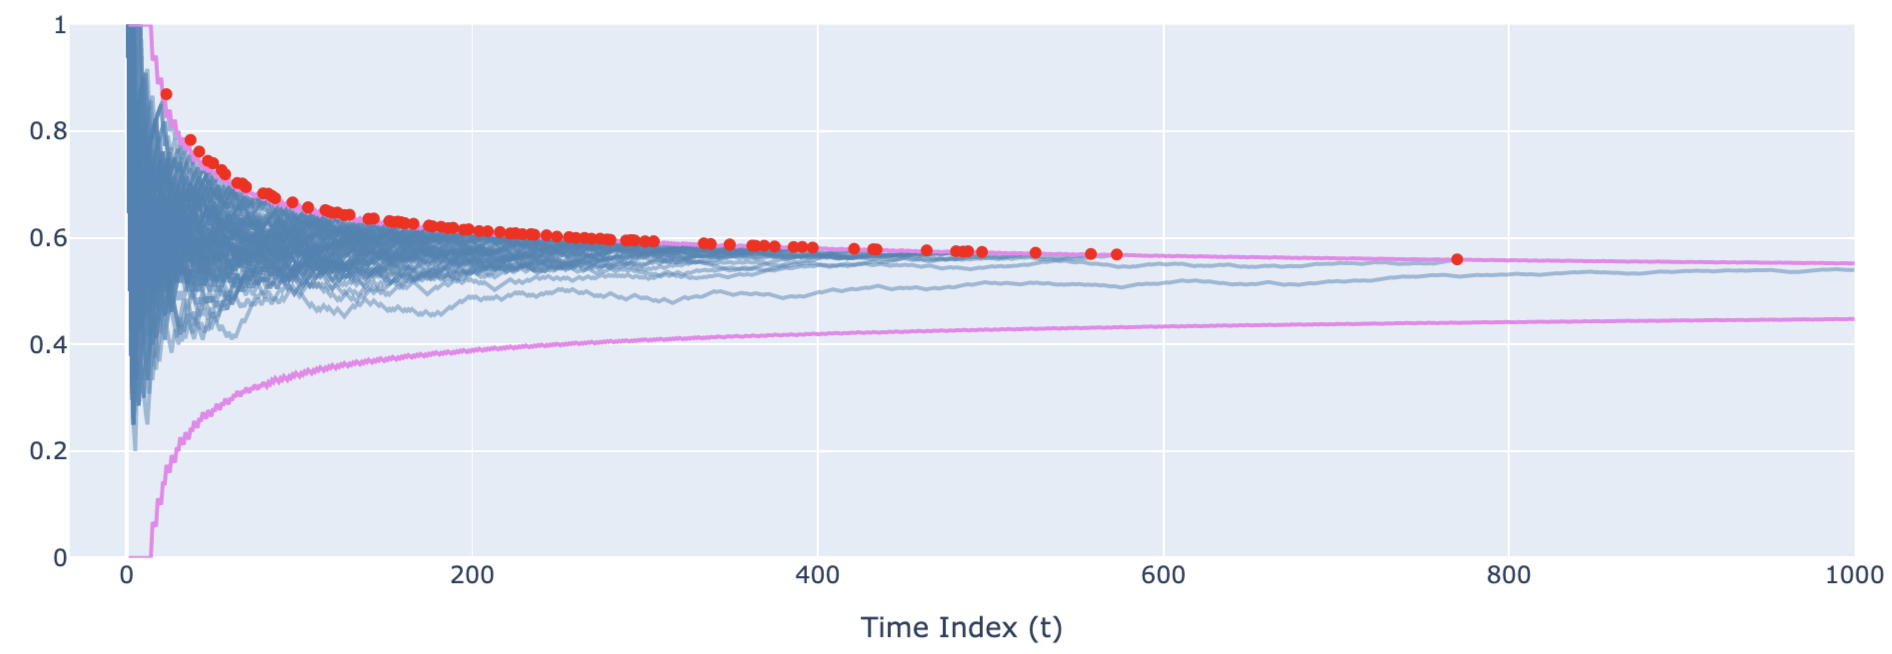
\includegraphics[scale=0.5]{images/ssrm_reject.png}
  \caption{Simulation Study of time to reject the null under the proposed test. The magenta curve is the same as in figure \ref{fig:critical}. Each blue trace is an independent simulation of $\hat{\rho}(x_{1:t})$ up until $t=1000$ or the first $t$ for which it crosses the rejection boundary of the Chi-squared test,visualized with a red dot, whichever comes sooner. }
    \label{fig:ssrm_reject}
  \end{figure}
  \noindent To add some intuition to figure \ref{fig:ssrm_reject}, it can be shown that the rection region at time $t$ converges to $[0,1]\setminus \theta_0$, yet $\theta_0 \rightarrow \theta_\star$ $a.s.$ as $t\rightarrow \infty$. In this specific example, the region of indifference degenerates onto $\lbrace 0.5 \rbrace$, yet $\hat{\rho}(x_{1:t})$ converges to 0.6 almost surely as $t \rightarrow \infty$ by the strong law of large numbers, which provides an alternative argument to theorem \ref{thm:consistency} for rejecting the null almost surely.
\section{Discussion}
The main purpose of this paper was to provide a tool that can be used sequentially to detect practical implementation errors in an experiment, such as identifying biased assignment mechanisms or surfacing missing data mechanisms which are frequently observed in online controlled experiments. The proposed test permits optional stopping and continuation, allowing experiments to be continuously monitored. The hypothesis can be tested, therefore, after every single data point so as to detect errors as quickly as possible. While Bayesian in construction, we provided sequential guarantees of the frequentist Type-I error probability and also studied the power of this test through a combination of theoretical results and simulation studies. While our application of detecting errors in simply randomized experiments focussed on a specific Multinomial-Dirichlet test, the same mathematical techniques can be obviously used to generalize these results to other Bayesian tests. With generalization in mind, there are some remaining comments and ideas for future work.

We first address the differences in the purely Bayesian approach and the test proposed here. For instance, under the same stopping rule of rejecting the null when the posterior odds exceed $1/u$, a Bayesian would report a (Bayesian) Type-I error probability of $u/(1+u)$, whereas a frequentist would report a slightly larger (frequentist) Type-1 error probability of $u$. One important distinction is that the latter does not depend at all on the realized data, whereas the former depends on the data actually observed. In this sense, the Bayesian answer is a data dependent error probability. The intuition that one is less likely to believe an outcome is a false positive as the test statistic becomes more extreme leads to the notion of conditional frequentist testing (\cite{kiefer}). In conditional frequentist testing one reports the data dependent Type-I error probability $\alpha(s) = \mathbb{P}(\text{Type I error} | S(X) = s)$ for a suitable conditioning statistic $S(X)$. The challenge in conditional frequentist testing is to find an appropriate conditioning statistic $S(X)$. \cite{conditional_frequentist_composite} showed that the Bayesian Type I error probabilities are equal to the conditional frequentist Type I error probabilities by choosing the conditioning statistic to be a function of the Bayes factor.

We note that the confidence sequences described in theorem \ref{thm:confidence_sequence} share a connection with other Bayesian intervals discussed in the literature. To see this it is necessary to express the Bayes factor in terms of the Savage-Dickey density ratio (\cite{dickey}) as
\begin{equation}
    B(x_{1:t}|\theta_0) = \frac{p(\theta_0| M_1)}{p(\theta_0|x_{1:t},M_1)}.
\end{equation}
This, with $O_0(\theta_0)=1$, implies that $I_t(u) = \lbrace \theta \in \mathbb{S}^d : O_t(\theta) \leq 1/u \rbrace = \lbrace \theta  \in \mathbb{S}^d : p(\theta| M_1)\leq p(\theta|x_{1:t}, M_1)/u \rbrace $, which is identified as the Bayesian \textit{support interval} proposed by \cite{support_interval}. The authors proposed this as an alternative to the more commonly reported Bayesian credible intervals, argueing that the support interval is based on evidence in the data (how the data changes belief), whereas credible intervals are based on posterior belief directly. These intervals have some intuitive appeal as they are the parameter values for which their posterior density has increased beyond some factor of their prior density after observing the data. We are the first, however, to identify the sequential frequentist coverage probabilities, in the sense of theorem \ref{thm:confidence_sequence}, of these support intervals.


\bibliographystyle{plainnat}
\bibliography{sample}


\appendix
\section{Posterior Odds Updating Rules}
\label{app:posterior_odds}
The Bayes factor after $t$ observations is analytically tractable, given by
\begin{equation}
  \label{eq:bayes_factor}
 \frac{p(x_{1:t}|M_1)}{p(x_{1:t}|M_0)} = \frac{\Gamma(\sum_{j=1}^{d} \alpha_j)}{\Gamma(\sum_{j=1}^{d} \alpha_j + \sum_{i=1}^{t}x_{i,j})}\frac{\prod_{j=1}^{d}\Gamma(\alpha_j + \sum_{i=1}^{t}x_{i,j} )}{\prod_{j=1}^{d}\Gamma(\alpha_j )}\frac{1}{\prod_{j=1}^{d} \theta_{0,j}^{\sum_{i=1}^{t}x_{i,j}}}.
\end{equation}
It is helpful to introduce some further notation to explicitly express the sequential nature inherent to the problem.

The Posterior odds in favour of $M_1$ to $M_0$ after observing $x_{1:t}$ is defined as
\begin{align}
  \label{eq:general_posterior_odds}
  \frac{p(M_1|x_{1:t})}{p(M_0|x_{1:t})}  &= \frac{\int p(x_{1:t}|\theta,M_1)p(\theta,M_1)d\theta}{p(x_{1:t}|M_0)}\frac{P(M_1)}{P(M_0)},\\
                      &=\frac{p(x_{1:t}|M_1)}{p(x_{1:t}|M_0)}\frac{p(M_1)}{p(M_0)},\\
                      &=\frac{\prod_{i=1}^{t}p(x_i|x_{1:i-1}|M_1)}{\prod_{i=1}^{t}p(x_i|x_{1:i-1}|M_0)}\frac{p(M_1)}{p(M_0)},\\
                      &=\frac{p(x_t|x_{1:t-1},M_1)}{p(x_t|x_{1:t-1},M_0)} \frac{p(M_1|x_{1:t-1})}{p(M_0|x_{1:t-1})},\\
    &=\frac{\int p(x_t|\theta,x_{1:t-1},M_1)p(\theta|x_{1:t-1},M_1)d\theta}{p(x_t|x_{1:t-1},M_0)}  \frac{p(M_1|x_{1:t-1})}{p(M_0|x_{1:t-1})} ,
\end{align}
where the last expression stresses the recursive definition of the Posterior odds factor in terms of products of posterior predictive densities. The posterior distribution of $\theta| x_{1:t}, M_1 \sim \text{Dirichlet}(\alpha_t)$ where $\alpha_t = \alpha_{t-1}+x_t$ with $\alpha_0$ the initial prior parameter choice. The posterior predictive densities are easily computed as
\begin{equation}
  \label{eq:posterior_predictive_m1}
   p(x_t|x_{1:t-1},M_1) = \frac{ \Gamma(\sum_i x_{t,i}+ 1)}{\prod_i \Gamma(x_{t,i} + 1)} \frac{\Gamma(\sum_i \alpha_{t-1,i})}{\prod_i \Gamma(\alpha_{t-1,i})} \frac{\prod_i \Gamma(\alpha_{t-1,i} + x_{t,i})}{\Gamma(\sum_i \alpha_{t-1,i} + x_{t,i})},
\end{equation}
and
\begin{equation}
  \label{eq:posterior_predictive_m2}
   p(x_t|x_{1:t-1},M_0) = \frac{ \Gamma(\sum_i x_{t,i} + 1)}{\prod_i \Gamma(x_{t,i} + 1)} \prod p_i^{x_{t,i}}.
 \end{equation}
 It will be useful later on to introduce the following notation for the posterior odds at time $t$ as $O_t(\theta_0)$, which explicitly states the value of $\theta$ under the null hypothesis. The recursive definition of the posterior odds can then be expressed as
\begin{align}
  O_{t}(\theta_0) &= \frac{\Gamma(\sum_i \alpha_{t-1,i})}{\Gamma(\sum_i \alpha_{t-1,i} +  x_{t,i})} \frac{\prod_i \Gamma(\alpha_{t-1,i} + x_{t,i})}{\prod_i \Gamma(\alpha_{t-1,i})} \frac{1}{\prod_i \theta_{0,i}^{x_{t,i}}}  O_{t-1}(\theta_0),\\
\end{align}
with
\begin{align}
  \label{eq:alpha_update}
  \alpha_{t}&= \alpha_{t-1}+x_t.
\end{align}
and initial value
\begin{align}
  \label{eq:bayes_factor_seed}
O_0(\theta_0) = \frac{p(M_1)}{p(M_0)}.
\end{align}


\section{Uniform Bounds on the Type-I Error}
\label{app:type_1_error}
To result follows from the application of the following two lemmas.
\begin{lemma}(Martingale property of posterior odds under the null hypothesis)
  
  \noindent Let $x_i,$ be a sequence of $\text{Multinomial}(n_i,\theta)$ random variables and consider the sequence of posterior odds $O_t(\theta_0)$ defined as in equation \eqref{eq:update_rule} with $O_0(\theta_0)=1$, then $O_t(\theta_0)$ is a nonnegative martingale under $M_0$.
  \label{lem:posterior_odds_martingale}
    \end{lemma}
  \begin{proof}
  \begin{align*}
    E_{M_0}[O_{t+1}(\theta_0)|\mathcal{F}_t]  &= \int \frac{p(x_{t+1}|x_{1:t},M_1)}{p(x_{t+1}|x_{1:t},M_0)} O_{t}(\theta_0) p(x_{t+1}|x_{1:t},M_0) d_{x_{t+1}}\\
    &=  O_{t}(\theta_0) \int p(x_{t+1}|x_{1:t},M_1) d_{x_{t+1}}\\
    &=  O_{t}(\theta_0),
  \end{align*}
  where $\mathcal{F}_{t} = \sigma(x_1,x_2,\dots, x_t)$
\end{proof}

\begin{lemma}(Ville's Maximal Inequality)
  
\label{lem:durrett}
  \noindent If $Z_{t}$ is a nonnegative supermartingale with respect to the filtration $\mathcal{F}_t$, then
  \begin{equation}
    \label{eq:durrett}
    \mathbb{P}[\exists t \in \mathbb{N}\cup \lbrace 0 \rbrace : Z_t \geq u] \leq \frac{Z_0}{u}
  \end{equation}
\end{lemma}
\begin{proof}
  See Proof 6.1 of \cite{howard}
\end{proof}
The result of the theorem is obtained by using lemma \ref{lem:posterior_odds_martingale} to establish that the posterior odds $O_t(\theta_0)$ are a nonnnegative supermartingale under the null hypothesis, and using this obseravtion in lemma \ref{lem:durrett} together with  $O_0(\theta_0) = 1$  to obtain the main inequality of the theorem.
\section{Asymptotic Properties of Bayes Factors}
\label{app:asymptotics}
We first narrow the focus of a general result found in theorem 1 of \cite{walker}. Let $D_{KL}(p(\cdot|\theta_\star)||p(\cdot|\theta) )$ denote the Kullback-Leibler divergence of a multinomial distribution indexed by a parameter $\theta$ from the true multinomial distribution with true parameter $\theta_{\star}$. Moreover let $D_{KL}(p(\cdot|\theta_\star)||p(\cdot|x_{1:t}, M_j) )$ denote the KL divergence of the posterior predictive distribution under model $j$ at time $t$ from the true multinomial distribution. Let $A(d) = \lbrace \theta \in \mathbb{S}^d : D_{KL}(p(\cdot|\theta_\star)||p(\cdot|\theta) ) < d \rbrace$
\begin{lemma}
  \label{lemma:walker}
  If $\int_{A(d)} p(\theta|M_j) > 0$ only for, and for all, $d > \delta_j$, and $\lim \inf_t D_{KL}(p(\cdot|\theta_\star)||p(\cdot|x_{1:t}, M_j) ) \geq \delta_j$ a.s. then
  \begin{equation}
    \label{eq:bayes_factor_convergence}
    \frac{1}{t} \log B_{10}(x_{1:t}) \rightarrow \delta_0 - \delta_1,
  \end{equation}
  provided that $\sum_t \frac{1}{t^2} \left( \mathbb{V}[\log \frac{p(x_t|x_{1:t-1},M_j)}{p(x_t|M_\star )}]\right) < \infty$.
\end{lemma}
\begin{proof}
  For a single model $j$, consider the following martingale
  \begin{align*}
    \label{eq:walker_martingale}
    S_{jt} =& \sum_{i=1}^{t} \log \frac{p(x_i|x_{1:i-1},M_j)}{p(x_i|M_\star)} + D_{KL}(p(\cdot|\theta_\star)||p(\cdot|x_{1:i-1}, M_j) ),\\
    =& -\log \frac{p(x_t|M_\star)}{p(x_t|x_{1:t-1},M_j)} + D_{KL}(p(\cdot|\theta_\star)||p(\cdot|x_{1:t-1}, M_j) ) +\\
    &S_{jt-1},\\
  \end{align*}
  from which it follows that $\mathbb{E}[S_{jt}|\mathcal{F}_t] = S_{jt-1}$ with $\mathcal{F}_t = \sigma(x_1,\dots,x_{t-1})$. From the assumption that  $\sum_t \frac{1}{t^2} \left( \mathbb{V}[\log \frac{p(x_t|x_{1:t-1},M_j)}{p(x_t|M_\star )}]\right) < \infty$, it follows that $S_{jt}/t \rightarrow 0$ a.s. and consequentially
  \begin{align*}
    \frac{1}{t} \frac{p(x_{1:t}|M_j)}{p(x_{1:t}|M_\star)} + \frac{1}{t}\sum_{i=1}^t  D_{KL}(p(\cdot|\theta_\star)||p(\cdot|x_{1:t-1}, M_j) )\rightarrow 0.
  \end{align*}
  From the additional assumption of $\lim \inf_t D_{KL}(p(\cdot|\theta_\star)||p(\cdot|x_{1:t}, M_j) ) \geq \delta_j$ a.s. , it follows that
  \begin{align*}
    \lim \sup   \frac{1}{t} \frac{p(x_{1:t}|M_j)}{p(x_{1:t}|M_\star)} \leq - \delta_j \hspace{1cm} a.s.
  \end{align*}
  With the Kullback Leibler property of the prior it follows that
  \begin{align*}
     \lim \inf   \frac{1}{t} \frac{p(x_{1:t}|M_j)}{p(x_{1:t}|M_\star)} \geq - \delta_j \hspace{1cm} a.s.
  \end{align*}
  from \cite{barron}. It follows that
    \begin{align*}
     \lim   \frac{1}{t} \frac{p(x_{1:t}|M_j)}{p(x_{1:t}|M_\star)} \rightarrow - \delta_j \hspace{1cm} a.s.
    \end{align*}
    Combining this result for models $M_1$ and $M_0$ completes the proof.
\end{proof}

The application of this lemma to the multinomial Dirichlet model is then straight forward. Note that under model $M_0$, the prior on $\theta$ is a point mass at $\theta_0$. Let the KL divergence of the null model from the true model be denoted $\delta_0$, it is clear that $\int_{A(d)} p(\theta|M_j) = 0$ if $d<\delta_0$ and 1 otherwise. Hence KL divergence of the null $\theta_0$ from the true $\theta_\star$ is the relevant $\delta_0$ for model $M_0$ in lemma \ref{lemma:walker}. The value of $\delta_1$ for the Dirichlet prior under model $M_1$, however, is zero. 
\end{document}